\SOL{

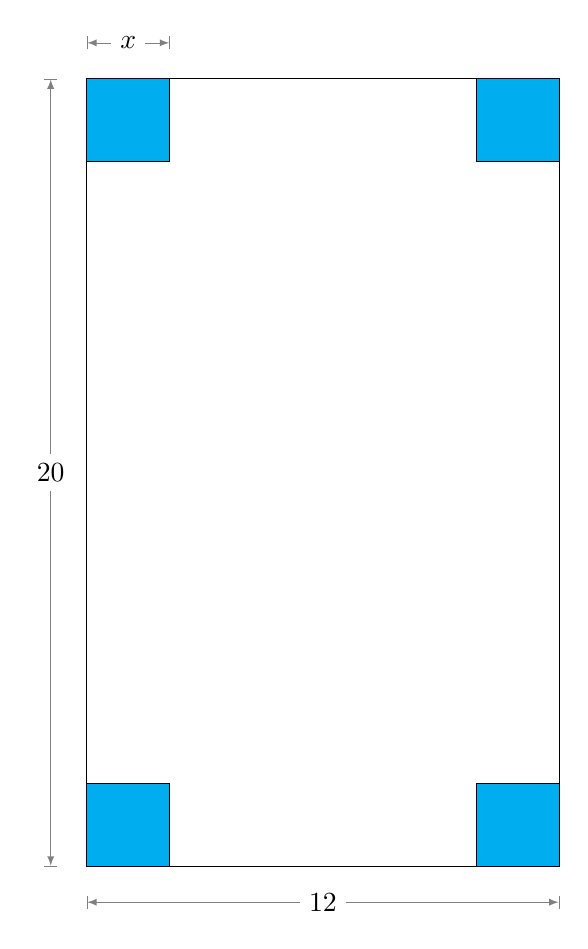
\begin{tikzpicture}[x=.5cm,y=0.5cm,>=latex]
\def\RWd{12}
\def\RHt{20}
\def\CutSide{30pt}
\draw
  (0,0) rectangle (\RWd,\RHt);
\path[draw,fill=cyan]
  (0,0) rectangle ++(\CutSide,\CutSide) 
  (\RWd,0) rectangle ++(-\CutSide,\CutSide) 
  (0,\RHt) rectangle ++(\CutSide,-\CutSide) 
  (\RWd,\RHt) rectangle ++(-\CutSide,-\CutSide);
\begin{scope}[|<->|,help lines,text=black]
\draw
  ([yshift=-13pt]0,0) -- node[fill=white] {$12$} ([yshift=-13pt]\RWd,0);   
\draw
  ([xshift=-13pt]0,0) -- node[fill=white] {$20$} ([xshift=-13pt]0,\RHt);   
\draw
  ([yshift=13pt]0,\RHt) -- node[fill=white] {$x$} ++(\CutSide,0);   
\end{scope}
\end{tikzpicture}

Para um determinado lado, devemos ter $x$ positivo 
\begin{eqnarray*}
		12-2x &>& 0\\
		-2x &>& -12\\
		2x &<& 12\\
		x &<& 6\\
\end{eqnarray*}
ou
\begin{eqnarray*}
		20-2x &>& 0\\
		-2x &>& -20\\
		2x &<& 20\\
		x &<& 10\\
\end{eqnarray*}

Em qualquer caso, $x$ deve ser positivo e menor que $6$, devemos ter: $x\in (0,6)$.

}
